\ylDisplay{Silinder} % Ülesande nimi
{Kaur Aare Saar} % Autor
{lõppvoor} % Voor
{2016} % Aasta
{G 4} % Ülesande nr.
{4} % Raskustase
{
% Teema: Dünaamika
\ifStatement
Silinder massiga $m$ ja raadiusega $R$ libiseb tasapinnal kiirusega  $v$ ja nurkkiirusega $\omega$. Kui libisemine on lõppenud, liigub silinder kiirusega $v$ esialgsega vastupidises suunas. Leidke silindri esialgne nurkkiirus.

\begin{center}
	\begin{resizebox}{0.35\linewidth}{!}{
			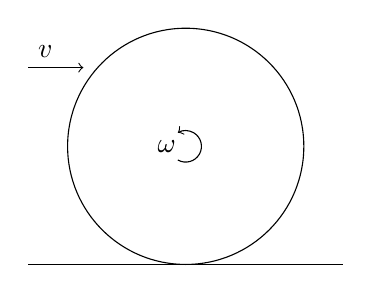
\begin{tikzpicture}
			\draw (0,2.5) node[anchor=south west] {$v$};
			\draw[->] (0,2.5) -- ++(0:0.7);
			\draw (0,0) --(4,0);
			\draw (2,1.5) circle (1.5);
			\draw [->] (2,1.5) node[anchor = east] {$\omega$} ++(-120:0.2) arc (-120:120:0.2);
			\end{tikzpicture}}
	\end{resizebox}
\end{center}
\fi


\ifHint
Silindri impulsimoment ei muutu telje suhtes, mis läbib silindri ja pinna kontaktpunkte, sest hõõrdejõul puudub jõuõlg selle telje suhtes.
\fi


\ifSolution
Silindri impulsimoment ei muutu telje suhtes, mis läbib silindri ja pinna kontaktpunkte, sest hõõrdejõul puudub moment selle telje suhtes. Olgu esialgne nurkkiirus $\omega$. Esialgne impulsimoment on seega $h_1=-mvR+I\omega=-mvR+mR^2\omega$, kus seest tühja silindri jaoks $I=mR^2$. Pärast libisemist on nurkkiirus $\frac{v}{R}$. Seega impulsimoment on $h_2=mvR+I\frac{v}{R}=2mvR$.
Impulsimomendi jäävusest $h_1=h_2$ saame, et $\omega=\frac{3v}{R}$.\\
\emph{Märkus.} Võis lahendada ka seest täis silindri jaoks. Siis $I=\frac{mR^2}{2}$ ja saame $\omega = \frac{5v}{R}$.
\fi


\ifEngStatement
% Problem name: Cylinder
A cylinder of mass $m$ and radius $R$ is sliding on a plane with a speed $v$ and an angular velocity $\omega$. When the sliding ends the cylinder moves with the speed $v$ to the opposite direction with respect to the initial speed. Find the cylinder’s initial angular velocity.
\begin{center}
	\begin{resizebox}{0.35\linewidth}{!}{
			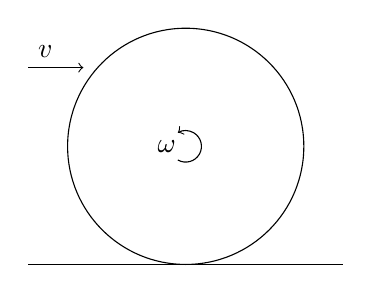
\begin{tikzpicture}
			\draw (0,2.5) node[anchor=south west] {$v$};
			\draw[->] (0,2.5) -- ++(0:0.7);
			\draw (0,0) --(4,0);
			\draw (2,1.5) circle (1.5);
			\draw [->] (2,1.5) node[anchor = east] {$\omega$} ++(-120:0.2) arc (-120:120:0.2);
			\end{tikzpicture}}
	\end{resizebox}
\end{center}
\fi


\ifEngHint
The angular momentum of the cylinder does not change with respect to the axis that goes through the contact points of the cylinder and the plane because the friction force is missing the respective torque arm.
\fi


\ifEngSolution
The cylinder’s angular momentum does not change with respect to the axis that goes through the contact points of the cylinder and the plane because friction does not have a torque with respect to this axis. Let the initial angular velocity be $\omega$. The initial angular momentum is therefore $h_1=-mvR+I\omega=-mvR+mR^2\omega$ where for a cylinder that is empty inside: $I=mR^2$. After the sliding the angular velocity is $\frac{v}{R}$. Therefore the angular momentum is $h_2=mvR+I\frac{v}{R}=2mvR$. From the conservation of angular momentum $h_1=h_2$ we get that $\omega=\frac{3v}{R}$.\\
\emph{Note}. This could have been solved for a filled cylinder as well. Then $I=\frac{mR^2}{2}$ and we get $\omega = \frac{5v}{R}$.
\fi
}